\newpage
\section{Projektowanie}		%3

\subsection{Środowisko i narzędzia programistyczne}
Proces projektowania i implementacji aplikacji został oparty o nowoczesny stos technologiczny zapewniający wydajność, skalowalność oraz zgodność ze standardami inżynierii oprogramowania:
\begin{itemize}
    \item \textbf{Język programowania:} C++ (w standardzie C++17/C++20), ze względu na pełną kontrolę nad zarządzaniem pamięcią oraz wsparcie dla paradygmatu obiektowego.
    \item \textbf{Środowisko programistyczne (IDE) i Kompilator:} Microsoft Visual Studio Community oraz natywny kompilator MSVC (\texttt{cl.exe}) wraz z narzędziem budującym \texttt{MSBuild}.
    \item \textbf{System kontroli wersji:} Git oraz platforma GitHub, służące do zarządzania historią kodu i pracy grupowej/eksperymentalnej.
    \item \textbf{Generator dokumentacji:} Doxygen, wspierający ustandaryzowany format komentarzy w kodzie źródłowym.
    \item \textbf{Dodatkowe biblioteki:} Standardowa biblioteka języka C++ (\textit{STL}), w tym nagłówki podstawowe takie jak \texttt{<iostream>}.
\end{itemize}

\subsection{Ustawienia kompilatora i konfiguracja projektu}
Kompilacja kodu źródłowego wymaga specyficznych flag konfiguracyjnych w celu zapewnienia poprawności działania programu, zwłaszcza w zakresie obsługi mechanizmów języka C++:
\begin{itemize}
    \item \textbf{Flaga obsługi wyjątków (\texttt{/EHsc}):} Kluczowy parametr kompilatora MSVC, który włącza standardową obsługę wyjątków synchronicznych (\textit{Exception Handling}). Umożliwia to poprawną konstrukcyjnie obsługę błędów alokacji pamięci oraz działania obiektów.
    \item \textbf{Architektura docelowa:} Projekt skonfigurowany jest dla architektury 64-bitowej (\texttt{x64}), co pozwala na pełne wykorzystanie przestrzeni adresowej nowoczesnych procesorów.
    \item \textbf{Konfiguracje budowania:} Wyróżnia się dwa główne warianty:
    \begin{itemize}
        \item \textit{Debug:} Zawiera symbole debugowania, wyłączone optymalizacje, przeznaczony do wykrywania błędów.
        \item \textit{Release:} Zoptymalizowany pod kątem wydajności i szybkości działania programu, z pominięciem metadanych diagnostycznych.
    \end{itemize}
\end{itemize}

\subsection{Architektura systemu i diagram klas (UML)}
Projekt zrealizowano w oparciu o cztery główne komponenty powiązane relacjami obiektowymi oraz wzorcami projektowymi:
\begin{enumerate}
    \item \textbf{Klasa \texttt{Node}:} Reprezentuje pojedynczy węzeł listy. Zawiera pole danych (\texttt{int data}) oraz wskaźniki na sąsiadów (\texttt{Node* next}, \texttt{Node* prev}).
    \item \textbf{Klasa \texttt{LinkedList}:} Główna struktura zarządzająca kolekcją. Przechowuje wskaźniki na początek (\texttt{head}) i koniec (\texttt{ogony/tail}) oraz aktualny rozmiar (\texttt{size}).
    \item \textbf{Klasa \texttt{ListIterator} (Wzorzec Iterator):} Odpowiada za sekwencyjny dostęp do elementów poprzez przeciążenie operatorów inkrementacji i wyłuskania.
    \item \textbf{Klasa \texttt{NodeFactory} (Wzorzec Fabryki):} Klasa pomocnicza zawierająca metodę statyczną odpowiedzialną za bezpieczne powoływanie do życia nowych instancji węzłów.
\end{enumerate}

Poniższy schemat tekstowy ilustruje powiązania pomiędzy strukturami w projekcie:

    \begin{figure}[!htb]
    	\begin{center}
    		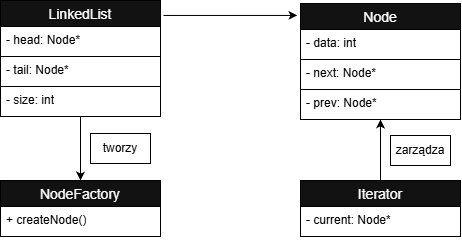
\includegraphics[width=0.8\linewidth]{rys/diagram1.png}
    		\caption{Schemat połączenia klas}
    		\label{rys:rysunek005}
    	\end{center}
    \end{figure}

\subsection{Sposób użycia systemu kontroli wersji (Git)}
W toku prac nad projektem wdrożono profesjonalny model Gałęzi (\textit{Branching Model}), co pozwala na bezpieczne wprowadzanie modyfikacji:
\begin{enumerate}
    \item \textbf{Główna gałąź (\texttt{main}):} Zawiera wyłącznie przetestowany, w pełni stabilny kod źródłowy oraz gotową aplikację.
    \item \textbf{Gałęzie testowe/robocze (np. \texttt{testowy-branch}):} Tworzone poleceniem \texttt{git checkout -b nazwa\_brancha} na potrzeby implementacji nowych wzorców (Iterator, Fabryka) lub modyfikacji algorytmów. 
    \item \textbf{Synchronizacja zmian:} Pozytywny wynik testów lokalnych skutkuje scaleniem kodu za pomocą polecenia \texttt{git merge} z gałęzią główną, a następnie przesłaniem zmian na zdalne repozytorium GitHub za pomocą \texttt{git push origin main}.
\end{enumerate}